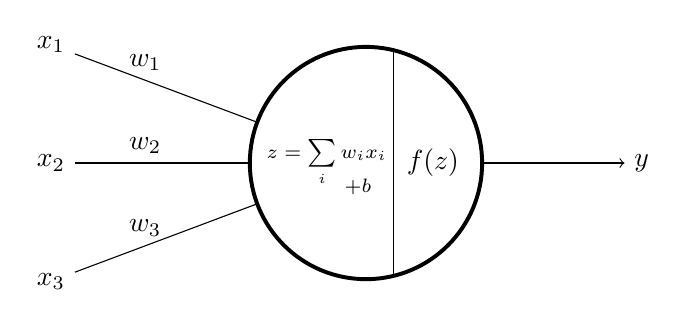
\begin{tikzpicture}
    \node[] at (-4,1.5) (a1) {\textbf{$x_1$}};
    \node[] at (-4,0) (a2) {\textbf{$x_2$}};
    \node[] at (-4,-1.5) (a3) {\textbf{$x_3$}};
    
    \node[] at (0,0) (b) {};
    
    \node[] at (3.5,0) (c) {\textbf{$y$}};  
    
	\path[->] (a1) edge node [near start,above] {$w_1$} (b);
	\path[->] (a2) edge node [near start,above] {$w_2$} (b);
	\path[->] (a3) edge node [near start,above] {$w_3$} (b);
    
    \path[->] (b) edge node [near start,above] {} (c);
    
    \path [draw=black,fill=white,line width=0.5mm] (0,0) circle (1.5cm-0.5\pgflinewidth);
    
%    \node[] at (-0.5,0.6) (b1) {$z$};
%	\node[rotate=90] at (-0.5,0.3) (b1) {$=$};
    \node[] at (-0.5,0) (b1) {{\scriptsize $z=\sum\limits_{i} w_i x_i$}};
    \node[] at (-0.1,-0.3) (b2) {{\scriptsize $ + b$}};
    
    \node[] at (0.35,1.57) (d1) {};
    \node[] at (0.35,-1.57) (d2) {};
    \path[] (d1) edge node [near start,above] {} (d2);
	\node[] at (0.85,0) (b3) {$f(z)$};
\end{tikzpicture}